\documentclass[a4paper,11pt, twoside]{report}
\usepackage[left=2.5cm,right=2cm,top=3cm,bottom=3cm]{geometry}

\usepackage{lipsum}
\usepackage{lineno}
\usepackage{etoolbox}
\usepackage[all]{xy}
\usepackage[english]{babel}
\usepackage{amssymb, amsmath} %math functions
\usepackage[T1]{fontenc}
\usepackage[utf8x]{inputenc}
\usepackage{url}

\usepackage{indentfirst}
\usepackage{listings}
\usepackage{multirow}
\usepackage{tabularx}
\usepackage{rotating} % for the rotated columns of table

% my imports
\usepackage{fancybox}
\usepackage{fancyhdr}
\usepackage{fancyvrb}
\usepackage{psboxit} % for the neat boxes on the footer
\usepackage{cite}
\usepackage[avantgarde]{quotchap}
\usepackage[english]{minitoc}
\usepackage{color,graphicx}
\usepackage[all]{xy}

%%%%%%%%%%%%%%%%%%%%%%%%%%%%%%%%%%%%
% DEFINE THE COLOR OF THE DOCUMENT
% use \def\bw{1} to generate the document in black and white
% \def\bw{1}
%%%%%%%%%%%%%%%%%%%%%%%%%%%%%%%%%%%%

\ifx\bw\undefined
\usepackage[pdfauthor={Ulisses Araujo Costa},
            urlcolor=darkblue,
            citecolor=darkblue,
            filecolor=darkblue,
            linkcolor=darkblue,
            pdftex,bookmarks,colorlinks,a4paper]{hyperref}
\else
\usepackage[pdfauthor={Ulisses Araujo Costa},
            urlcolor=black,
            citecolor=black,
            filecolor=black,
            linkcolor=black,
            pdftex,bookmarks,colorlinks,a4paper]{hyperref}
\fi
% end notes package (the second one --- hyperendnotes is for use hyperref with endnotes)
\usepackage{endnotes,chngcntr}
\usepackage{hyperendnote}

\usepackage{pifont} % for \cross symbol newcommand
\usepackage{subfig}
\usepackage{graphicx}

\usepackage[acronym,shortcuts]{glossaries}
\makeglossaries

\definecolor{darkblue}{rgb}{0,0,0.6}
%\renewcommand\familydefault{\sfdefault}% usar font sem serifas
\pdfpagewidth=\paperwidth
\pdfpageheight=\paperheight

%%%%%%%%%%%%%%%%%%%%%%%%%%%%%%%%%%%%%%%%%%%%%%%%%%%%%%%%%%%%%%%%%%%%%%%%%%%%
\lstdefinelanguage{codeTTN}
{
        basicstyle=\ttfamily\footnotesize,
        sensitive=true,
        showstringspaces=false,
        numberblanklines=true,
        showspaces=false,
        breaklines=true,
        showtabs=false,
		numbers=left,
		numberstyle=\footnotesize,
		xleftmargin=15pt,
		captionpos=b % caption below :)
}
\lstnewenvironment{code}[1][]{\lstset{language=codeTTN,caption=#1}}{}
%%%%%%%%%%%%%%%%%%%%%%%%%%%%%%%%%%%%%%%%%%%%%%%%%%%%%%%%%%%%%%%%%%%%%%%%%%%%
\ifx\bw\undefined
\newcommand{\checkK}{\color{green}\checkmark}
\newcommand{\cross}{\color{red}\hspace{-3pt}\ding{55}}
\newcommand{\bigexclaim}{\color{yellow}$\bigtriangleup$\hspace{-5.6pt}!}
\else
\newcommand{\checkK}{\color{black}\checkmark}
\newcommand{\cross}{\color{black}\hspace{-3pt}\ding{55}}
\newcommand{\bigexclaim}{\color{black}$\bigtriangleup$\hspace{-5.6pt}!}
\fi
%%%%%%%%%%%%%%%%%%%%%%%%%%%%%%%%%%%%%%%%%%%%%%%%%%%%%%%%%%%%%%%%%%%%%%%%%%%%
%% first reset the headers and footers

\fancyhead{}
\fancyfoot{}
%% make the odd pages have the section name on the top right
\fancyhead[RO]{\sffamily\bfseries \rightmark}
%% make the even pages have the chapter name on the top left
\fancyhead[LE]{\sffamily\bfseries \leftmark}

%% page nums on the bottom in a nice box
%% even side pages
\fancyfoot[LE]{\psboxit{box 0.8 setgray fill}
{\framebox[10mm][c]{\rule{0cm}{4mm}\color{black}{\bfseries \thepage}}}}
%% odd side pages
\fancyfoot[RO]{\psboxit{box 1 setgray fill}
{\hspace{\textwidth}\psboxit{box 0.8 setgray fill}
{\framebox[10mm][c]{\rule{0cm}{4mm}\color{black}{\bfseries \thepage}}}}}

%% make the bottom line above the page number box
\renewcommand{\footrulewidth}{0.4pt}
\renewcommand{\footruleskip}{0mm}

\pdfpagewidth=\paperwidth
\pdfpageheight=\paperheight

\pagestyle{fancy}
%%\lhead{}
%%\rhead{}

%% now redefine the plain style pages (chapter pages, contents pages)
%% to have the same page number stuff on the bottom
\fancypagestyle{plain}{}
%	\fancyhf{}
%	\fancyfoot[RO]{\psboxit{box 1 setgray fill}
%	{\hspace{\textwidth}\psboxit{box 0.8 setgray fill}
%	{\framebox[10mm][c]{\rule{0cm}{4mm}\color{black}{\bfseries \thepage}}}}}
%	\renewcommand{\headrulewidth}{0pt}
%	\renewcommand{\footrulewidth}{0.5pt}
%}

%% this next section (till \makeatother) makes sure that blank pages
%% are actually completely blank, cause they're not usually
\makeatletter
\def\cleardoublepage{\clearpage\if@twoside \ifodd\c@page\else
	\hbox{}
	%\vspace*{\fill}
		\phantom{}
	\thispagestyle{empty}
		\vfill
		\vfill
	\newpage
	\if@twocolumn\hbox{}\newpage\fi\fi\fi}
\makeatother
%%\parindent=0pt
%%\parskip=4pt
%%%%%%%%%%%%%%%%%%%%%%%%%%%%%%%%%%%%%%%%%%%%%%%%%%%%%%%%%%%%%%%%%%%%%%%%%%%%
%%%%%%%%%%%%%%%%%%%%%%%%%%%%%%%%%%%%%%%%%%%%%%%%%%%%%%%%%%%%%%%%%%%%%%%%%%%%
%%%%%%%%%%%%%%%%%%%%%%%%%%%%%%%%%%%%%%%%%%%%%%%%%%%%%%%%%%%%%%%%%%%%%%%%%%%%

%% stuff do minitoc %%%%%%%%%%%%%%%%%%%%%%%%%%%%%%%%%%%%%%%
\setcounter{minitocdepth}{2}
\setlength{\mtcindent}{24pt}
\renewcommand{\mtcfont}{\small\rm}
\renewcommand{\mtcSSfont}{\small\bf}
\renewcommand{\mtctitle}{Contents of chapter \thechapter}
%\newenvironment{mtc}{\secttoc\sectlof\sectlot}{\pagebreak}
%                        ^       ^        ^
%                    conteudos  figuras  tabelas
% \newenvironment{mtc}{\minitoc\minilof\minilot}{\pagebreak}
%%%%%%%%%%%%%%%%%%%%%%%%%%%%%%%%%%%%%%%%%%%%%%%%%%%%%%%%%%%

%%%%%%%%%%%%%%%%%%%%%%%%%%%%%%%%%%%%%%%%%%%%%%%%%%%%%%%%%%%%%%%%%%%%%%%%%%%%%%%%%%
% A Black page with a message in the middle: "This page intentionally left blank"
%%%%%%%%%%%%%%%%%%%%%%%%%%%%%%%%%%%%%%%%%%%%%%%%%%%%%%%%%%%%%%%%%%%%%%%%%%%%%%%%%%
\newcommand{\blankpage}
	{
		\thispagestyle{empty}
		\phantom{}
		\vfill
		\begin{center}{\centering This page intentionally left blank}\end{center}
		\vfill
		\newpage
		\addtocounter{page}{-1}
	}

%%%%%%%%%%%%%%%%%%%%%%%%%%%%%%%%%%%%%%%%
% Author notes
%%%%%%%%%%%%%%%%%%%%%%%%%%%%%%%%%%%%%%%%
\def\note#1{{\noindent {\color{red}\textbf{NOTA:} #1}}}
% New Content
\newcommand{\new}[1]{{\linenumbers\color{blue}#1}}
%\newcommand{\new}[1]{{#1}}

%%%%%%%%%%%%%%%%%%%%%%%%%%%%%%%%%%%%%%%%
%%% ACRONYM (GLOSSARY)
%%%%%%%%%%%%%%%%%%%%%%%%%%%%%%%%%%%%%%%%
% List of Acronyms leged
\newcommand{\listofacronymsname}{List of Acronyms}
% remove the dot (.) at the end of a glossary entry...
\renewcommand*{\glspostdescription}{}

%%%%%%%%%%%%%%%%%%%%%%%%%%%%%%%%%%%%%%%%
%%%%%%%%%%%%%%% ENDNOTES %%%%%%%%%%%%%%%
%%%%%%%%%%%%%%%%%%%%%%%%%%%%%%%%%%%%%%%%
% Replace all footnotes by endnotes
\let\footnote=\endnote
\let\theendnotee=\theendnote
% Section of endnotes (at the end of a chapter usually)
\newcommand{\secendnote}{
	% If we don't have footnotes in a chapter, don't print the footnotes listing
	\ifnum\value{endnote}=0
	\else
		\newpage
		\begingroup
		\parindent 0pt
		\parskip 2ex
		\def\enotesize{\normalsize}
		\def\notesname{Notes of chapter \arabic{chapter}}
		\def\theendnote{\arabic{chapter}.\theendnotee} %2.1 note menas that is the first note (1) from chapter 2 :)
		\theendnotes
		\endgroup
	\fi
}
% Reset endnote numbering every new chapter
\counterwithin{endnote}{chapter}

%listings
\renewcommand*{\lstlistlistingname}{List of Listings}

%%%%%%%%%%%%%%%%%%%%%%%%%%%%%%%%%%%%%%%%%%%%%%%%%%%%%%%%%%%%%%%%%%%%%%%%%%%%%%%%
%%%%%%%%%%%%%%%%%%%%%%%%%%%%%%%%%%%%%%%%%%%%%%%%%%%%%%%%%%%%%%%%%%%%%%%%%%%%%%%%
%%% BEGIN OF LaTeX DOCUMENT
%%%%%%%%%%%%%%%%%%%%%%%%%%%%%%%%%%%%%%%%%%%%%%%%%%%%%%%%%%%%%%%%%%%%%%%%%%%%%%%%
%%%%%%%%%%%%%%%%%%%%%%%%%%%%%%%%%%%%%%%%%%%%%%%%%%%%%%%%%%%%%%%%%%%%%%%%%%%%%%%%
\begin{document}
\pagenumbering{roman}
\newcommand{\newac}[2]{\newacronym{#1}{#1}{#2}}

\newac{SIMSAT}{Simulation Infrastructure for the Modeling of SATellites}
\newac{SMP}{Simulation Model Portability}
\newac{ESA}{European Space Agency}
\newac{MMI}{Man Machine Interface}
\newac{GSTV}{Ground Systems Test and Validation Applications}
\newac{OMG}{Object Management Group}
\newac{MDA}{Model Driven Architecture}
\newac{UML}{Unified Modeling Language}
\newac{XML}{eXtensible Markup Language}
\newac{VST}{VisionSpace Technologies}
\newac{UM}{University of Minho}
\newac{ECSS}{European Cooperation for Space Standardization}
\newac{CFG}{Control Flow Graph}
\newac{VDM}{Vienna Development Method}
\newac{ADL}{Assertion Definition Language}
\newac{SAT}{Satisfiability}
\newac{JML}{Java Modeling Language}
\newac{ACSL}{ANSI/ISO C Specification Langage}
\newac{AST}{Abstract Syntax Tree}
\newac{GCC}{GNU C Compiler}
\newac{ESOC}{European Space Operations Centre}
\newac{IBM}{International Business Machines Corporation}
\newac{AsmL}{Abstract State Machine Language}
\newac{API}{Application Programming Interface}
\newac{LLVM}{Low Level Virtual Machine}
\newac{OO}{Object Oriented}
\newac{OCL}{Object Constraint Language}
\newac{SDO}{Standard Development Organizations}
\newac{HB}{Handbook}
\newac{TM}{Technical Memoranda}
\newac{GUI}{Graphical User Interface}
\newac{BSSC}{Board for Software Standardisation and Control}
\newac{RTCA}{Radio Technical Commission for Aeronautics}
\newac{EUROCAE}{European Organisation for Civil Aviation Equipment}
\newac{ISO}{International Organization for Standardization}
\newac{SQA}{Software Quality Assurance}


\thispagestyle{empty}
\begin{center}
\begin{tiny}.\end{tiny}\\
\vspace{3.5cm}
\begin{huge} University of Minho \end{huge} \\
\vspace{0.3cm}
\begin{LARGE} Department of Informatics \end{LARGE} \\
\vspace{5cm}

\begin{large}
\textbf{Title}\\
\vspace{0.2cm}
by\\ 
\vspace{0.2cm}
Ulisses Araújo Costa\\
\end{large}

\vspace{8cm}
Submitted in partial fulfilment of the requirements for the \\
MSc Degree in Informatics of University of Minho\\
\vspace{2cm}
Date\\
\end{center} 

\chapter*{Acknowledgements}

%I would like to thank first of all to my supervisor, Dr Nicholas John Dingle, as he was the main source of guidance, information and help throughout the whole duration of the Project Background Paper and Final Project Report here presented.\\

%Secondly, I would like to show my appreciation to all my family that always supported me emotionally and financially whilst I was pursuing my MSc.\\

%Finally, to all my Imperial College class mates and to those other friends or colleagues that were a source of joy, happiness and inspiration during the last academic year, hereby I thank you all.\\


\chapter*{Resumo}

%I would like to thank first of all to my supervisor, Dr Nicholas John Dingle, as he was the main source of guidance, information and help throughout the whole duration of the Project Background Paper and Final Project Report here presented.\\

%Secondly, I would like to show my appreciation to all my family that always supported me emotionally and financially whilst I was pursuing my MSc.\\

%Finally, to all my Imperial College class mates and to those other friends or colleagues that were a source of joy, happiness and inspiration during the last academic year, hereby I thank you all.\\
Lorem ipsum dolor sit amet, consectetur adipiscing elit. Suspendisse suscipit, quam dapibus suscipit gravida, felis purus tincidunt orci, sit amet fringilla turpis lacus vel turpis. Aenean sem mi, pretium ac gravida id, adipiscing ac tortor. Maecenas pellentesque diam pellentesque risus lacinia ac ullamcorper enim blandit. Nulla eu ante sollicitudin turpis sodales viverra nec at erat. Phasellus cursus congue nisl, non ornare massa volutpat in. Fusce diam quam, blandit at pretium sit amet, commodo egestas metus. Donec lorem sem, imperdiet eget semper et, convallis ultrices lorem. Sed euismod, lorem non blandit porta, orci augue varius velit, nec blandit urna nibh vel sapien. Nunc dictum velit vel sem laoreet tempor.

\cleardoublepage
\chapter*{Abstract}
\ac{ESA} uses a big engine to perform tests in the
Ground Segment infrastructure, specially the Operational Simulator.
This engine uses many different tools to ensure the development of
regression testing infrastructure and these tests perform black-box
testing to the C++ simulator implementation.
\ac{VST} is one of the companies that provides
these services to \ac{ESA} and they need a tool to instead of writing
manually scripts to perform tests, it should try to automatically
infer tests from the existing C++ code.
There are many approaches trying to tackle this problem and therefore
many tools were developed. Here we will present a study on the most
recent tools that uses: Model-based testing, Specification-based
testing, Constraint-based generation, Random generation and
Grammar-based generation for the most used languages - C, JAVA and C\#.

Automated Test Case Generation tools give support for creating test
cases and at the same time ensure test case coverage methodically. The
main goal of this tools is extract information from the program on how
to generate executable test cases.
Using manual written tests is tedious, time consuming and error-prone.
Lots of functions/methods need full code coverage and this technique
leaves to incomplete test suites and is hard to create tests that
cover specific code paths potentially leaving many hidden bugs.
Besides that, software is not a static artifact and is constantly
evolving, so a test generation technique could be a more suitable
mechanism in the development process.
We will be mainly focused on the white-box automatic test generation techniques.

Since no other testing tool used by \ac{ESA} makes any use of a formal
model we decide to start by infer the \ac{UML} model from the existing C++
code and try to explore the generation of \ac{OCL} specifications
from C++ code and \ac{UML} diagrams. The idea is to capture the requirements properties about the code, and from this beef up the white-box automatic test generation.



\dominilof \dominilot \dominitoc
\cleardoublepage \tableofcontents   \addcontentsline{toc}{chapter}{\contentsname}
\cleardoublepage \listoftables      \addcontentsline{toc}{section}{\listtablename}
\cleardoublepage \listoffigures     \addcontentsline{toc}{section}{\listfigurename}
\cleardoublepage \lstlistoflistings \addcontentsline{toc}{section}{\lstlistlistingname}
% Print Glossary into the document
\newpage
\addcontentsline{toc}{section}{\listofacronymsname}
\printglossary[
	 type=\acronymtype
	,style=listdotted
	,title={\listofacronymsname}
	,toctitle={\uppercase{\listofacronymsname}}
	]
% Start the thesis
\newpage
\pagenumbering{arabic}
\addtocounter{mtc}{+1} %fix the minitoc numbering
\ifx\neat\undefined
\begin{savequote}[10pc]
{%
\parindent 0pt
\ifx\preLilyPondExample \undefined
\else
  \expandafter\preLilyPondExample
\fi
\def\lilypondbook{}%

\includegraphics[width=3.5\textwidth]{images/bachPrelude}
\ifx\postLilyPondExample \undefined
\else
  \expandafter\postLilyPondExample
\fi
}
\qauthor{Cello Suite No.1 i-Prelude, Johann Sebastian Bach}
\end{savequote}
\fi
\chapter{Introduction}
\minitoc

\new{
With the increasing size and complexity of software systems, modeling techniques related to abstraction\cite{dicsbuchs06}
and decomposition\footnote{Decomposition, also known as factoring, is the process of break down a complex system
into parts that are easier to conceive, understand, program, and maintain.}\cite{struct-analy} of the system has
shown to be very important\cite{dicsbuchs06}.
These techniques allow an early vision of the software to be developed, allowing analysis and previous evaluation before
the model be implemented.
Because of this, the use of software models in the process of developing a software system is very important regarding
the organization of the activities in order to obtain high quality at lower cost.
In this context, the \ac{UML} is the standard language, used for modeling the structure of software projects.\\
Since ever, every industry use testing methods to discover problems in early stages of the development process to improve
the products quality, and software industry is not an exception. Software testing became an essential method for software quality assessment and became
widely used and accepted for the validation and verification of software systems. It can be considered as a complete revision
of the specification, design and implementation of a software system.
}
Miller\cite{miller} describe the utility of software testing as:

\begin{quotation}
The general aim of testing is to affirm the quality of software systems by systematically
exercising the software in carefully controlled circumstances.
\end{quotation}

In the most recent period of software history the integration of
software testing as an important step in the process of
software development opened up to the origin of xUnit\cite{xunit}
tools and Agile software development.
Also, \ac{ESA} started to use manual written tests as a part of their
software development processes.\\
Using  manual written tests is tedious, time consuming and error-prone.
Lots of functions/methods need full code coverage and this practice
leads to incomplete test suites;
as it is hard to create tests that cover specific code paths, many
hidden bugs can be left.
Many times a supervision leaded by the developer
is needed to assure that the right paths in the code are being tested,
specially regarding black-box testing.\\
Nowadays we start to observe a rapid increase in the automatic test
generation field.

\section{Operational Simulator Infrastructure}
\ac{ESA}'s Operational Simulator called \ac{SIMSAT}
is a satellite simulator that model and simulate
the behavior of satellites in order to allow operators\footnote{Operators are responsible for the operation of the satellite after its launch.} train more effectively 
and help them to define the satellites' operational processes.

The simulator consists of operational models of the various internal components of the satellite from their main computer to its payload (instruments aboard the satellite),
which interact with each other and thus define the behavior of the satellite.
\ac{VST} has participated in the development of tests to validate the operational simulator.
The development of these simulators is based on operating rules simulation of
\ac{ESA} -- \ac{SMP}\footnote{\ac{SMP} is based on the ideas of component-based design and \ac{MDA}
as promoted by the \ac{OMG} and is based on the open standards of \ac{UML} and \ac{XML}.
One of the basic principles is the separation of the platform specific and platform independent aspects of the simulation model.
This protects the investments in the model from changes in technology by defining the model in a platform independent way, which can then be mapped into different technologies.
Further the \ac{SMP} specification provides standardized interfaces between the simulation models and the simulation run-time environment for common simulation services as well as a
number of mechanisms to support inter-model communication.\cite{1A,2A,3A,4A,5A}}, as well as in infrastructure \ac{SIMSAT} simulation.
This standard is infrastructure agnostic of any space specific model, so any other needs of simulation can be used, such as defense, transport, energy, etc.\\
\ac{SIMSAT}\footnote{More information in: \url{http://www.egos.esa.int/portal/egos-web/products/Simulators/simsat/intro-sim.html}} is composed by $6$ parts:
\ac{SIMSAT} Kernel is a generic simulation infrastructure that provides the framework to run space systems simulations.
\ac{SIMSAT} \ac{MMI} is a generic \ac{GUI} enabling the user interaction with the simulator's components.
Ground Models are a family of \ac{SIMSAT} compatible models enabling a realistic simulations of all ground systems between the spacecraft (or spacecraft model)
and the control center at \ac{ESOC}\cite{Martin_whitepaper}. These modules are standard and include implementation of uplink and downlink processors.
Emulator Suite On-board Processor Emulators support the execution in satellite simulators of the real flight software.
Generic Models a set of generic space models that ease the developments of the spacecraft models used in operational simulators.
\ac{GSTV} this is a family of test simulators that are based on the generic simulators infrastructure components listed above and are able to support the different levels
of testing of ground infrastructure systems.\\

The \ac{SIMSAT} Kernel is the part we are interested in performing automatic test generation, because is the main component regarding the simulation.
The Kernel is made up of several components\footnote{More information in: \url{http://www.egos.esa.int/portal/egos-web/products/Simulators/SIMSAT/}} including
a Scheduler that is responsible for the co-ordination and processing of all events within the Simulation Kernel.
An event on the schedule identifies an action that needs to be performed at a specified point in simulated time.\\
A Mode Manager that is the simulation state machine. The Simulation has a number of operational modes, which control the operation of the simulation.\\
The Time-Manager that is responsible for maintaining and providing models and the \ac{MMI} with the correct simulation-Time,
it provides time in four formats, Simulation-Time, Epoch-Time, Zulu-Time and Correlated Zulu-Time, this is a family of \ac{SIMSAT}
compatible models enabling a realistic simulations.\\
The Logger supports the recording of Kernel or model events that occur during a simulation.
The log in which the current simulation messages are written is called the active log.
The logger also provides a view of the simulation event history in an \ac{MMI} during a simulation session.\\
The Visualization manager is responsible for making the values of both model and Kernel data items available for display in an \ac{MMI}.
State-vector manager is responsible for the saving and restoring of the state of the simulation. Its main purpose is to allow the Simulation State, at any point in the simulation, to be saved. This allows the user to return to an earlier simulation scenario.\\
Command handler is responsible for the reception and execution of Kernel and user defined commands.a set of generic space models that ease the developments of the spacecraft models used in operational.\\
Command procedure interpreter is responsible for the interpretation of command procedures.
A command procedure contains Kernel and User defined simulator commands and supports a procedural language to control the flow of these commands.
The execution of command procedures is controlled directly from the \ac{MMI}\cite{1996ESASP.394..399L}.

Right now, to be able to perform tests in the Operational Simulator, in order to validate \ac{SIMSAT}, \ac{VST} Engineers need to write scripts that
perform simulations and validate the results using \ac{GUI} (\ac{SIMSAT} \ac{MMI}). This job can be tedious and difficult to replicate.\\
So a first solution will have to go through a preliminary study of the tools
that currently exist with which we can generate tests automatically.
By studding these tools we do not hope to find the perfect solution, but combine techniques to obtain an optimal solution to improve \ac{VST} work.
\section{Goals}
This document correspond to the first milestone in the author's dissertation (developed under a partnership agreement between \ac{UM} and \ac{VST}) aimed at producing a tool
that is able to automatically generate interesting testcases for the C++ \ac{ESA}'s Operational Simulator.\\
This document reviews the most studied techniques
and the tools that implement them in order to choose the best set of
suitable techniques to incorporate in an automatic
testing generator to the Ground Segment infrastructure, specially the
Operational Simulator at \ac{ESA}.\\
Two different techniques emerge for different purposes, Structural
Techniques and Functional Techniques,
known respectively as White-box\cite{stt} testing and Black-box\cite{black} testing.
Functional testing is the most common at \ac{ESA}, because of the
calculation complexity behind the Operational Simulators.\\
A brief discussion will be presented regarding White-box testing vs. Black-box
testing and then some automatic generation techniques will be discussed in more detail.
Furthermore the potential of the described tools will be explained, and how they can help
on solving the problem \ac{VST} has nowadays. First of all an explanation about the Operational Simulator Infrastructure will be provided.

\section{Contribution}
\note{Falar nos resultados atingidos}
\section{Document Outline}
\note{Falar no forma como os capitulos se organizam e sugerir formas de leitura}\\
At the beginning of each chapter there will be a brief explanation about the chapter content and at
the end a summary is provided in order to sum up the explained content.\\

Moreover at the beginning of each chapter there is a mini table
of contents showing the whole structure and location of all sections and subsections within that chapter.
Each chapter notes will be shown at the end of the chapter in a separate section called "Notes of chapter $c$" where $c$ is the chapter number,
in order to facilitate reading throughout the full page while not restricting the size of the notes.
Each note is referenced with the format $X.Y$ meaning that
the note $Y$ belongs to chapter $X$.
\secendnote

\chapter{Testing}
\minitoc
In this chapter are discussed and contextualized historically the \ac{ECSS} standards by which the space industry is governed (Section \ref{sec:historyspace} and Section \ref{sec:doc-stand}).
The importance of this Standards is addressed regarding the security of the software products for space purposes, it is also
shown the classification of \ac{ECSS} software criticality (Section \ref{sec:stand}) and starting therefrom are shown testing techniques that 
respond to such high requirements, with the aim to analyze the code coverage (Section \ref{sec:ccoverage}).
\new{
Related to space Standards it is also shown the most reliable Standard for airborn software components -- The DO-178/ED-12 from \ac{EUROCAE} and \ac{RTCA} (Section \ref{sec:airborne}).
Also it will be shown the most recent version of this Standard and the relationship between it and \ac{ECSS} software Standards (Section \ref{sec:new-stand}).\\
The expression "safety" will be used in terms of a property of a system that it will not endanger human life or the environment and
the expression "safety-critical" is used to describe a
system that is intended to achieve, on its own, the necessary level of safety integrity for the implementation of the required safety functions.
So, a safety-critical software is an artifact that if
fails can cause loss of human life or have other catastrophic consequences.\\
}
In a second part of this chapter the main differences between White-box and Black-box testing are presented and
some testing tools approaches are described considering automatic generation testing techniques, and some tools for each technique namely:
Specification-based Generation Testing, Constraint-based Generation Testing, Grammar-based Generation Testing and
Random-based Generation Testing.
\section{ESA and ECSS Standardization in Space Industry}
Software products for space industry tends to be a part of a network composed by several systems. This space systems include manned and unmanned spacecraft,
launchers, payloads, experiments and their associated ground equipment and facilities\cite{Mattiello-FranciscoSanAmbJogCos:2007:BrSoIn}.
These kind of projects are generally  expensive, demand considerable amount of time to be completed and have different companies and countries participating.\\
Trying to get a Standard way to follow all rules to deliver the components with the same degree of quality and reliability is extremely important.\\

Software development for Space, particularly in Europe, follows very specific rules on international standards. These standards not only define how a software project should
evolve but also how every component developed in the field of Space Industry should be done, tested, documented, deployed and maintained.
This include not only software but many more artefacts like: Electrical, Mechanical and Material components, etc.\\
In 1994, \ac{ECSS} was established to develop a single set of consistent Space standards recognized and accepted for use by the entire European Space Community.
\ac{ECSS} is supported by \ac{ESA} Council deliberations since the foundation and has developed, through
a partnership between \ac{ESA}, National Space Agencies and European Industry, the management and implementation of European Space Projects.\\
The main objectives of \ac{ECSS} are to increase the effectiveness of all Space programmes in Europe through the application of a
single, integrated set of Standards and Requirements from which all generic requirements of future Space projects can be derived and
improve the competitiveness of the European Space industry.
This is particularly important to formalize an unambiguous communication in order to facilitate the interaction between project partners,
create a set of legally binding documents, reduce risks, guarantee interface compatibility and
improve the quality and safety of Space projects and products.\\
In section \ref{sec:historyspace} we will see the history of Space Industry Standards and the need for them.

\subsection{History of Software Development Standards for Space Industry}\label{sec:historyspace}
\ac{ESA} Software Engineering Standards originate around 1975. At
that time the \ac{ESA} was working on a number of ambitious projects, on relatively new subjects, involving the development of
large amounts of code. The project teams often consisted of technically excellent engineers, but most of them were not used to work in projects with
rigorous cost and a strict schedule. There was very little project oriented discipline\cite{esa-bulletin-90}.\\

One of the projects had a high level of criticality (as we will see later on Table \ref{tab:severity}) and the
development activity was done at \ac{ESOC}, namely to support the mission, the launch of which was imminent.
The project began delaying and there were some major hardware, operating system problems. The team was waiting for improvements in the hardware
and eventually to be able to continue the work, they reduced the amount of requirements to only
those highly essential for the launch of the satellite. The problem was faced when they realize that no one knew the exact system requirements.
\begin{quotation}
There were no written requirements — at best, some could partly be
retrieved from minutes of meetings. All the rest were in the minds of the project engineers. How
could cost and schedule be guaranteed under these circumstances? This was a project manager's
worst nightmare!\cite{esa-bulletin-90}
\end{quotation}

The team manager decided to stop any further development. All software engineers write down their understanding of the requirements.
As they had a written list of requirements, they were now able to select only
those requirements needed for the launch. The remaining requirements were implemented after
the satellite was launched. In this case a disaster was prevented from happening\cite{Zwartjes05anagile}.
The \ac{BSSC} was subsequently founded in order to \ac{ESA} never end up in an identical situation. This was the seed from
which the \ac{BSSC}, and consequently, the \ac{ESA} Software Engineering Standards was funded and prospered.\\
\ac{ESA}'s \ac{BSSC} was formally established in May 1977 ant it was defined that \ac{BSSC} responsibilities were to:
\begin{itemize}
\item Establish and maintain engineering standards for the procurement, development and maintenance of software.
\item Verify that the standards thus established are made applicable to software
development activities at \ac{ESA}. The \ac{BSSC} verifies the application of the PSS-05-0\cite{pss-05-0} standards through a procedure involving the
scrutiny of contracts with a software content.
These rather limited controls have succeeded remarkably well in helping to instill a software standards "culture" within the organisation.
\item Act as liaison with \ac{ESA} Legal Affairs department concerning the safeguarding of intellectual
property rights relating to software.
\end{itemize}
PSS-05-0 was a very successful Standard and \ac{BSSC} has played an important role in promoting it, both through its various
publications and through its responsibility in monitoring its application. PSS-05-0 has served to create a common software engineering culture in \ac{ESA}\cite{esa-bulletin-90}.\\
In June 1994, \ac{ESA} Council confirmed the willing to transfer the present PSS system of \ac{ESA} space standards to a new system
of standards, today known as \ac{ECSS}, in order to expand the Standards 
to other European national space agencies and European space industry in general.
The \ac{ECSS} system of standards covers a bigger area, as we explain before: management, product assurance and engineering standards, specifically for space projects.
The \ac{ECSS} Standard for software engineering, ECSS-E-40\cite{ecss-e-st-40c}, is a high-level requirements-oriented standard, in effect a tailoring of ISO/IEC 12207 for space projects.
Unlike the old PSS-05-0, it reflects the specifics of space projects, for example the relationship between the space system development cycle and the software development cycle\cite{esa-bulletin-90}.

\subsection{Document Standards}\label{sec:doc-stand}
ECSS-S-ST-00\cite{ecss-s-st-00c} document is the top level user document of \ac{ECSS}.
It gives a general introduction into \ac{ECSS} and the correct use of \ac{ECSS} Documents in space
programmes and projects.
Its purpose is to provide users with an overview of the \ac{ECSS} System, together
with an introduction to the three branches of applicability, (that will be explained later on this section) and to the disciplines
covered by the set of \ac{ECSS} Standards and the processes involved in generating
and using these standards.
In this document there is also an introduction into space programmes, space projects actors and their
customer-supplier relationships. The application of this System for space projects in the customer-supplier
chain is also explained and a practical tailoring method is described together with
methods for collecting and processing user feedback.
Finally the top-level requirements are defined for implementation of the \ac{ECSS}
system in space projects/programmes\cite{ecss-s-st-00c}.\\

Under this document there are three parallel branches, the branche dedicated to project management,
engineering, and product assurance.
Project management branch documents have an "M" prefix, engineering standards have an "E" prefix, and product assurance standards have a "Q" prefix.
Within each branch, disciplines and corresponding requirements are covered by dedicated standards.
Standards are normative document written specifically for direct use in invitation to tender and 
business agreements for implementing space related activities. Its content 
is strictly limited to the statement of verifiable customer requirements, supported 
by the minimum descriptive text necessary for understanding their context.

\ac{ECSS} Disciplines can also be supported by \ac{HB} and \ac{TM} as necessary\cite{ecss-s-st-00c}.
\ac{HB} are non-normative document providing orientation, 
guidelines, technical data, advice or recommendations, which contains 
information about how to implement space related activities. There are two types of \ac{HB}'s: Guidelines and good practices and Collection of data.
On the other side, \ac{TM} are non-normative documents providing useful information to the space community 
on a specific subject, prepared to record and present non-normative data, which 
are not relevant for a Standard or for a \ac{HB}, or not yet mature to be published as \ac{HB} or standard.

In order to clear understand the disciplines addressed by the \ac{ECSS} Standards system,
is shown in Figure \ref{fig:ecssdocsstruct} the Standard document by \ac{ECSS} where it is possible to clearly
see the three separated branches (M, E and Q)\cite{ecss-s-st-00c}.
It is also possible to see standards from other \ac{SDO} that are integrated into \ac{ECSS} new standards.

\def\a{\save[].[dddddd]!C="a"*[F--]\frm{}\restore}
\def\b{\save[].[dddddddd]!C="b"*[F--]\frm{}\restore}

\def\h{\save[].[rr]!C="h"*+<7pt>+[F:<100pt>]\frm{}\restore}

\ifx\bw\undefined
\begin{figure}[!ht]
\footnotesize
\begin{displaymath}
\xymatrix@=.28cm{
  & *+[F-]{\txt{ECSS-S-ST-00\cite{ecss-s-st-00c} - ECSS System}} \ar@{->}[d] \ar@{->}[dl] \ar@{->}[dr] & \\
	\h\a{\txt{Space project management\\(management Standards)}}
  & \b{\txt{Space product assurance\\(product assurance Standards)}}
  & \b{\txt{Space engineering\\(engineering Standards)}} & *+[F]{\txt{External\\standards\\adopted by\\ECSS}}\ar@/{}_{3pc}/@{->}[];"h"+<3.1pt,28.3pt>+\\
	*+[F**:red]{\txt{M-10 - Project planning\\and implementation}}
  & *+[F**:blue][white]{\txt{Q-10 - Product\\assurance management}}
  & *+[F**:green]{\txt{E-10 - System\\engineering}}\\
	*+[F**:red]{\txt{M-40 - Configuration and\\information management}}
  & *+[F**:blue][white]{\txt{Q-20 - Quality assurance}}
  & *+[F**:green]{\txt{E-20 - Electrical and\\optical engineering}}\\
	*+[F**:red]{\txt{M-60 - Cost and schedule\\management}}
  & *+[F**:blue][white]{\txt{Q-30 - Dependability}}
  & *+[F**:green]{\txt{E-30 - Mechanical\\engineering}}\\
	*+[F**:red]{\txt{M-70 - Integrated logistic\\support}}
  & *+[F**:blue][white]{\txt{Q-40 - Safety}}
  & *+[F**:green]{\txt{E-40\cite{ecss-e-st-40c} - Software\\engineering}}\\
	*+[F**:red]{\txt{M-80 - Risk management}}
  & *+[F**:blue][white]{\txt{Q-60 - EEE components}}
  & *+[F**:green]{\txt{E-50 - Communications}}\\
  & *+[F**:blue][white]{\txt{Q-70 - Materials, mechanical\\parts and processes}}
  & *+[F**:green]{\txt{E-60 - Control\\engineering}}\\
  & *+[F**:blue][white]{\txt{Q-80\cite{ecss-q-st-80c} - Software\\product assurance}}
  & *+[F**:green]{\txt{E-70 - Ground systems\\and operations}}\\
  & & &
}
\end{displaymath}
    \caption{ECSS System}\label{fig:ecssdocsstruct}
\end{figure}

%documneto que define o sistema ecss\cite{ecss-s-st-00c}
%documento de qualidade\cite{ecss-q-st-80c}
%ulisses paper\cite{costa_et_al:OASIcs:2012:3523}
\else
\begin{figure}[!ht]
\footnotesize
\begin{displaymath}
\xymatrix@=.28cm{
  & *+[F-]{\txt{ECSS-S-ST-00\cite{ecss-s-st-00c} - ECSS System}} \ar@{->}[d] \ar@{->}[dl] \ar@{->}[dr] & \\
	\h\a{\txt{Space project management\\(management Standards)}}
  & \b{\txt{Space product assurance\\(product assurance Standards)}}
  & \b{\txt{Space engineering\\(engineering Standards)}} & *+[F]{\txt{External\\standards\\adopted by\\ECSS}}\ar@/{}_{3pc}/@{->}[];"h"+<3.1pt,28.3pt>+\\
	*+[F]{\txt{M-10 - Project planning\\and implementation}}
  & *+[F]{\txt{Q-10 - Product\\assurance management}}
  & *+[F]{\txt{E-10 - System\\engineering}}\\
	*+[F]{\txt{M-40 - Configuration and\\information management}}
  & *+[F]{\txt{Q-20 - Quality assurance}}
  & *+[F]{\txt{E-20 - Electrical and\\optical engineering}}\\
	*+[F]{\txt{M-60 - Cost and schedule\\management}}
  & *+[F]{\txt{Q-30 - Dependability}}
  & *+[F]{\txt{E-30 - Mechanical\\engineering}}\\
	*+[F]{\txt{M-70 - Integrated logistic\\support}}
  & *+[F]{\txt{Q-40 - Safety}}
  & *+[F]{\txt{E-40\cite{ecss-e-st-40c} - Software\\engineering}}\\
	*+[F]{\txt{M-80 - Risk management}}
  & *+[F]{\txt{Q-60 - EEE components}}
  & *+[F]{\txt{E-50 - Communications}}\\
  & *+[F]{\txt{Q-70 - Materials, mechanical\\parts and processes}}
  & *+[F]{\txt{E-60 - Control\\engineering}}\\
  & *+[F]{\txt{Q-80\cite{ecss-q-st-80c} - Software\\product assurance}}
  & *+[F]{\txt{E-70 - Ground systems\\and operations}}\\
  & & &
}
\end{displaymath}
    \caption{ECSS System}\label{fig:ecssdocsstruct}
\end{figure}
\fi

The application of this Standards regarding space related projects is not a strict imposition, they enforce
tailoring to the technical, cost, schedule, programmatic and economic characteristics of the space programmes and projects.
For a specific project, Standards are tailored according to all the traits of the project: the type and 
phase of the project, the acceptable risks, the project complexity, cost, etc.
So, tailoring is the process by which individual requirements are evaluated and made applicable to a specific project.
The available list of standards and their content is analysed in order to select the set of standards to be made applicable to the project, taking 
into account its specificity and constrains and identify those requirements in the individual standards which are not 
applicable to the project, modify or exceptionally add requirement for specific needs\cite{ecss-s-st-00c}.
Tailoring is an important task in order to deliver a suitable product or service considering the costumer needs.

\subsection{ECSS-Q-80 and Testing}\label{sec:stand}
Software development projects tend to be specific depending on the application domain and 
space software projects are not an exception. These projects tend to have particular dynamics than software projects
in other domains because space software development pose additional challenges due to its inherent
requirement that the end products should be highly dependable.
The criticality factor of those systems (sometimes life critical) tend to have different more stringent requirements and approaches 
compared to less critical software projects, so
the existing software engineering standards are not enough to cope with these challenges, this is why \ac{ECSS} has developed a set of standards for European
space projects\cite{Ahmad2010AgileECSS,10.1109/SESS.1997.595952}.
This is why \ac{ECSS} have a particular E branch Standard completely dedicated to "Software Product Assurance" --- The ECSS-Q-80\cite{ecss-q-st-80c}.\\

The fundamental principle of these Standard is to facilitate the
customer-supplier relationship assumed for all software developments, at all levels.
They have contributed to these objectives by providing a set of requirements to be
met throughout the system lifetime which involves the development and
maintenance of space application software. Such requirements deal with quality
management, lifecycle activities and process definition, and quality
characteristics of the software product\cite{Mattiello-FranciscoSanAmbJogCos:2007:BrSoIn}.
Therefore the main objective of this Standard is to provide the customer with adequate confidence about the software product.\\

In order to improve greater security in the code that is produced for space industry, the Standard ECSS-Q-80\cite{ecss-q-st-80c} defines
some levels of criticality of the software, depending on their use in the mission.
This categorization is separate into 4 levels (A,B,C and D) regarding what can happen if the software fails or if it is not executed.
In the following listing we can see the classification:

\begin{description}
\item[Level A] Software that if not executed, or not correctly executed, or if anomalous behaviour can cause or contribute to a system failure resulting in \textbf{Catastrophic consequences};
\item[Level B] Software that if not executed, or not correctly executed, or if anomalous behaviour can cause or contribute to a system failure resulting in \textbf{Critical consequences};
\item[Level C] Software that if not executed, or not correctly executed, or if anomalous behaviour can cause or contribute to a system failure resulting in \textbf{Major consequences};
\item[Level D] Software that if not executed, or not correctly executed, or if anomalous behaviour can cause or contribute to a system failure resulting in \textbf{Minor or Negligible consequences}.
\end{description}

Each Severity level is intrinsically connected to a level of safety into the mission. Catastrophic corresponds to
Loss of life, life-threatening or permanently disabling injury or occupational illness; Loss of system; 
Loss of an interfacing manned flight system; Loss of launch site facilities; and Severe detrimental environmental effects. The result
of having a software component fail within this level leaves to major failures propagation in the mission\cite{ecss-q-st-30c}.\\
The Critical level corresponds to Temporarily disabling but not life-threatening injury, or temporary occupational illness;
Major damage to interfacing flight system; Major damage to ground facilities; Major damage to public or private property;
and Major detrimental environmental effects. The result of having a software component fail this level leaves to loss of mission.\\
The other two levels: Major and Minor leaves to Major mission degradation and Minor mission degradation with no or negligible safety results in the mission.
In Table \ref{tab:severity} we have the \ac{ECSS} Severity Classification of consequences information summarized acording to \cite{ecss-q-st-40c}.
According to the standard
when several categories can be applied to the system or system component, the highest severity takes priority.
\begin{table}[!ht]
\centering
\noindent \begin{tabular}{|c|c|m{4cm}|m{5cm}|}\hline
\textbf{Severity} & \textbf{Level} & \textbf{Dependability (from \cite{ecss-q-st-30c})} & \textbf{Safety}\\\hline\hline
\multirow{5}{*}{\textbf{Catastrophic}} & \multirow{5}{*}{$1$} & \multirow{5}{*}{Failures propagation} & 
Loss of life, life-threatening or permanently disabling injury or occupational illness;\\\cline{4-4}
& & & Loss of system;  \\ \cline{4-4}
& & & Loss of an interfacing manned flight system; \\ \cline{4-4}
& & & Loss of launch site facilities;  \\ \cline{4-4}
& & & Severe detrimental environmental effects.  \\\hline\hline
\multirow{5}{*}{\textbf{Critical}} & \multirow{5}{*}{$2$} & \multirow{5}{*}{Loss of mission} & 
Temporarily disabling but not life-threatening injury, or temporary occupational illness;\\\cline{4-4}
& & & Major damage to interfacing flight system;  \\ \cline{4-4}
& & & Major damage to ground facilities; \\ \cline{4-4}
& & & Major damage to public or private property;  \\ \cline{4-4}
& & & Major detrimental environmental effects.  \\\hline\hline
\textbf{Major} & $3$ & Major mission degradation & --\\\hline\hline
\textbf{Minor} & $3$ & Minor mission degradation or any other effects & --\\\hline
\end{tabular}
\caption{ECSS Severity Classification of consequences}\label{tab:severity}
\end{table}

To ensure more security about the source code, regarding the severity level, \ac{ECSS} standards, namely \cite{ecss-q-st-40c}
consider the application of formal tools to verify the source code. But at the same time, a major emphasis to software testing.
\ac{ECSS} divides the the test effort regarding the criticality of the source code.
If the source code is classified as Level A then the tests for that piece of software should meet 100\% in
three different categories: Source code statement coverage, Source code decision coverage and Source code modified condition and decision coverage.\\
Statement coverage measure the part of the program within which every executable source code statement has been invoked at least once.
Decision coverage measure of the part of the program within which every point of entry and exit
is invoked at least once and every decision has taken TRUE and FALSE
at least once (this includes statement coverage).
Modified condition and decision coverage measure of the part of the program within which every point of entry and exit
has been invoked at least once, every decision in the program has taken TRUE and FALSE values at least once, and each condition in a decision has been
shown to independently affect that decision's outcome. A condition is shown to independently affect a
decision's outcome by varying that condition while holding fixed all other possible conditions. All of these code coverages will be explained in more detail in section
\ref{sec:ccoverage}\\
If the source code is classified as Level B then the tests for that piece of software should meet 100\% in the first two categories of testing and should be
agreed with the costumer the value for to meet regarding Source code modified condition and decision coverage.
If the source code is classified as Level C or D then the tests for all the three categories should be agreed with the costumer.
In the following Table \ref{tab:ccoverage} this information is summarized.

\begin{table}[!ht]
\centering
\noindent \begin{tabular}{|m{6cm}|c|c|c|c|}
\hline
\textbf{Code Coverage vs. Criticality} & A & B & C & D \\\hline
Source code statement coverage & 100\% & 100\% & AM & AM \\\hline
Source code decision coverage & 100\% & 100\% & AM & AM \\\hline
Source code modified condition and decision coverage & 100\% & AM & AM & AM \\\hline
\multicolumn{5}{|m{14cm}|}{
NOTE: "AM" means that the value is agreed with the customer and measured for:
unit level testing; integration level testing and validation against the
technical specification and validation against the requirements baseline
as in \cite{ecss-q-st-80c} at clause 6.3.5.2.
}\\\hline
\end{tabular}
\caption{ECSS Code Coverage vs. Criticality}\label{tab:ccoverage}
\end{table}

\new{
\section{DO-178/ED-12 Standard for Airborne Systems}\label{sec:airborne}
Software in avionics has been around since 1970's, but was in the 80's when the cost of computers went down, thanks to the introduction of personal computers,
that the avionics industry start to use software components in airborne systems.
The increased use of Software and Computer systems for safety-critical applications motivated the development in 1980 of
DO-178 by \ac{RTCA}
\footnote{
\ac{RTCA} is a US non-profit organization that develops technical guidance for use by government regulatory authorities and by industry.
The documents it publishes are treated as guidelines, not as requirements.\\
\ac{RTCA}'s objectives are to:
\begin{itemize}
\item Ensure the safety and reliability of airborne systems;
\item Develop minimum operational performance requirements for document-specific systems;
\item Develop guidelines for use by a regulatory authority;
\item Provide administrative and logistics resources that enable teamwork among the world-wide aviation community.
\end{itemize}
}
and ED-35 by \ac{EUROCAE}
\footnote{
\ac{EUROCAE} has now been operating for more than 40 years as a non-profit organization
whose membership exclusively comprises aviation stakeholders made up of Manufacturers,
Services Providers, National and International Aviation Authorities and Users (Airlines, Airports, operators) from Europe.
}
leading to the creation of a single Standard and some years later in 1985 --- The DO-178/ED-12 Standard: The first
common certification criteria for production of avionics software. This document has the title
"Software Considerations in Airborne Systems and Equipment Certification" and became a worldwide basis for software
certification in the aviation industry until nowadays. This Standard is
officially recognized as a \textit{de facto} international Standard by the \ac{ISO} for software certification in the aviation industry.\\
Compared to other Software Standards like MIL-STD-498, MIL-STD-2167A, IEEE/EIA-12207, IEC 61508 all of these standards deal with certain aspects of
software development covered by DO-178/ED-12\cite{ed-12b} and none of them has been found to provide a complete coverage of Software Development process as DO-178/ED-12 do
\cite{avionics}.

One of the things that these documents defined was the Software Levels\cite{ed-12b}, ie DO-178/ED-12 requires that all systems requirements be mapped
to one of the five software levels:
\begin{description}
\item[Level A] Most critical failure level. Failure at Level A results in catastrophic failure conditions for an aircraft;
\item[Level B] The software at this level contributes to severe-major failure conditions;
\item[Level C] Software at this level contributes to major failure conditions;
\item[Level D] Software at this level contributes to minor failure conditions;
\item[Level E] The software has no effect toward potential failure conditions.
\end{description}
As we have seen in section \ref{sec:stand}, this classification is very similar.
The fact is that this Standard has served as initial motto for ECSS-Q-80\cite{ecss-q-st-80c} and ECSS-E-40\cite{ecss-e-st-40c}, \ac{ECSS} standards.
In fact \ac{ECSS} software standards were naturally fetched from many learned lessons in avionics.
Many other definitions in \ac{ECSS} ECSS-Q-80\cite{ecss-q-st-80c} and ECSS-E-40\cite{ecss-e-st-40c} were drawn based on DO-178/ED-12, like the
Severity classification of consequences, code covera vs. Criticality and many more guidelines.

DO-178/ED-12 has three Software Life cycle Processes where are defined the objectives of each step in the software development as well
the set of activities for meeting the objectives:
\begin{description}
\item[Software Planning Process] where the Standard defines five types of planning data\footnote{\ac{RTCA} and \ac{EUROCAE} avoid referring to this "data" as
"documents" when trying to elaborate on the objective evidence that need to be produced to satisfy the Standard objectives\cite{avionics}, on the other side \ac{ECSS} refers
these evidences as "documents". So we can consider these evidences as documents.} that should include
considerations on the methods, languages, standards and tools to be used during the development phase. These plans are: Plan for Software Aspects of Certification,
Software Development Plan, Software Verification Plan, Software Configuration Management Plan and Software Quality Assurance Plan.
\item[Software Development Process] where the Standard defines that should be included the requirements, that can be
expressed as high- and low-level requirements\cite{avionics,ed-12b}. The Standard allow the system complexity and the design methodology applied to the system under development
drive the requirements decomposition process. The design, coding and integration artifacts are briefly described since these tend to vary between various development methodologies.
However the Standard defines clearly the expected outputs of each of the processes, the design process yields low-level requirements and software architecture.
The coding process produces the source code, in a high-order language or assembly code. The integration process result in executable code
resident on the target computer. The Standard also predicts that each of these outputs should be verified, assured and configured.
\item[Integral Process] Four processes are defined as integral in DO-178/ED-12 which
mean that they can be overlaid and extended throughout the
software life cycle. They are as follows:
\begin{itemize}
\item Software Verification: Verification is the most important
in DO-178/ED-12 which accounts to over two thirds of the total.
\item Software Configuration Management: The clear definition
of what is to be verified will be more reasonable for the
various outputs of the verification in DO-178/ED-12. This definition
or configuration is the design of the DO-178/ED-12 objectives
for configuration management.
\item Software Quality Assurance: \ac{SQA} objectives provide oversight of the entire DO-178/ED-12
process and require independence at all levels. \ac{SQA} guarantees
detection of plans and standards, deviated during development
process are recorded, evaluated, tracked and resolved.
\item Certification Liaison Process: As mentioned earlier, the
issues should be identified early for the certification process.
DO-178/ED-12 outlines twenty data items to be produced in a
compliant process where three of these are specific to it and
must be provided to the certifying authority: Plan for Software Aspects of Certification, Software Configuration Index and Software Accomplishment Summary.
\end{itemize}
\end{description}
\subsection{The new Standard DO-178C/ED-12C}\label{sec:new-stand}
The first version of DO-178/ED-12 was DO-178A/ED-12A and was released in 1985 and twenty years later the Standard had a new update -- The DO-178B/ED-12B released in 1992,
ten more years and in 2012 the most recent version of the Standard was released following the existing nomenclature: DO-178C/ED-12C.
The most recent version of the Standard takes into account new technologies and methodologies developed since 1992 (the previous version of the Standard).
These methodologies and Technologies include the \ac{OO} Paradigm, Model based design/automatic code generators and \ac{RT} operating systems.
The new Standard also recognize that there is more to software verification than testing \textit{per se} and includes Formal methods\cite{Brosgol:2011:DNA:2070337.2070341} and abstract interpretation
and also takes into account the supplementary papers/commentaries on DO-178B.\\
The most recent version includes three supplements: 
\begin{description}
\item[ED-216 Formal Methods] identifies the additions, modifications and substitutions to ED-12C and ED-109A objectives when formal methods are used as part of a software life cycle, and the additional guidance required. It discusses those aspects of airworthiness certification that pertain to the production of software, using formal methods for systems approved using ED-12C;
\item[ED-217 Object-Oriented Technology and related techniques] identifies the additions, modifications and deletions to ED-12C and ED-109A objectives 
when \ac{OO} technology or related techniques are used as part of the software development life cycle and additional guidance is required.
This supplement, in conjunction with ED-12C, is intended to provide a common framework for the evaluation and acceptance of \ac{OO} technology
and related techniques \ac{RT}-based systems;
\item[ED-218 Model-Based development and verification] contains modifications and additions to ED-12C and ED-109A. Objectives, activities, explanatory text and
software life cycle data that should be addressed when model-based development and verification are used as part of the software life cycle.
This includes the artifacts that would be expressed using models and the verification evidence that could be derived from them.
Therefore, this supplement also applies to the models developed in the system process that define software requirements or software architecture.
\end{description}

The benefits of incorporating the \textbf{ED-216 Formal Methods} supplement are important because
the use of mathematical models, that defines the system using an unambiguous abstraction syntax (eg state machines, Z notation, set theory, \ac{DSL}'s),
and mathematical analysis, that provides guarantees/proofs of software properties regarding the compliance with requirements,
may be applied at various stages during the software development and can be used as a formal verification technique.
This supplement sees Formal methods as a complement to testing, basically testing shows that functional requirements
are satisfied and sometimes is able to detect errors and Formal methods can increase confidence that no anomalous behavior will occur
(formal methods may found faults that are not detected by testing techniques)\cite{Chelini:2009:WTD:1647420.1647443}.\\
The benefits from incorporating the \textbf{ED-217 Object-Oriented Technology and related techniques} supplement are important because
it assumes that \ac{OO} paradigms bring more safety to software development than other lower level languages once massively used in aerospace.
The Data-centric approach of \ac{OO} languages eases maintenance of many large systems, the use of Model-driven architecture tool (like \ac{UML}) facilitates
the generation of \ac{OO} code\cite{Elliott:2010:OSC:1869542.1869558}. The use of a Standard paradigm allow space industry to use languages used by many programmers such as C++, JAVA or Ada95.
The features that this paradigms bring to space software are very important, namely, the capability of Method overloading, the type conventions, the re-use of
generic templates, exceptions and concurrency, etc.\\
The benefits from incorporating the \textbf{ED-218 Model-Based development and verification} supplement are essentially the motivation to use unambiguous notation and supports the use of
automated code generation tools, namely automatic test generation tools\cite{Chelini:2009:WTD:1647420.1647443}. This supplement acknowledges the need of
high-level requirements from which development model is derived and the ability to demonstrate properties for the model, showing that the property 
is preserved in the source code.\\

As we can see the Standard ECSS-Q-80\cite{ecss-q-st-80c} in the software quality assurance side and ECSS-E-40\cite{ecss-e-st-40c} in the software development side
gives a distinguished emphasis on software validation and verification, however is the Standard DO-178/ED-12, for reasons obvious,
that gives much more emphasis in the verification component. The biggest proof is the most recent embedding of the Formal Methods into the
new version of the Standard DO-178C/ED-12C\cite{ed-12c}, in order to reach where the tests are not enough.
Increasingly the use of tools and methodologies from the area of Formal Methods is crucial to prevent software errors and ensure quality and their proper functioning.

\section{Code Coverage}\label{sec:ccoverage}
As we have seen previouslly, code coverage is a major concern regarding the software development for space industry, it is very important to provide a study on this subject
in order to access a possible integration of this feature into the final product.

\cite{ccoverage}
\cite{mcdc}
\cite{Marick99}
%\note{
%Nesta seccao pretendo falar com grande detalhe nas varias vertendes de code coverage tendo em consideracao os standards da ECSS.
%Como por exemplo: Statement Coverage, Decision Coverage, Condition Coverage, Multiple Condition Coverage, Condition/Decision Coverage,
%Modified Condition/Decision Coverage, Path Coverage.\\
%E ainda Function Coverage, Call Coverage, Linear Code Sequence and Jump (LCSAJ) Coverage, Data Flow Coverage, Object Code Branch Coverage,
%Loop Coverage, Race Coverage, Relational Operator Coverage, Weak Mutation Coverage, Table Coverage
%}
%\subsection{Statement Coverage}
%\subsection{Decision Coverage}
%\subsection{Condition Coverage}
%\subsection{Multiple Condition Coverage}
%\subsection{Condition/Decision Coverage}
%\subsection{Modified Condition/Decision Coverage}
%\subsection{Path Coverage}
%\subsection{Function Coverage}
%\subsection{Call Coverage}
%\subsection{Linear Code Sequence and Jump (LCSAJ) Coverage}
%\subsection{Data Flow Coverage}
%\subsection{Object Code Branch Coverage}
%\subsection{Loop Coverage}
%\subsection{Race Coverage}
%\subsection{Relational Operator Coverage}
%\subsection{Weak Mutation Coverage}
%\subsection{Table Coverage}
}
\section{White-box vs Black-box testing}
%In this section is discussed the two most common approaches for testing: White-box and Black-box testing.\\
In White-box testing the tester needs to understand the internals of
the code to be able to write tests for it.
The goal of selecting test cases that test specific parts of the code
is to cause the execution of specific spots in the software, such as
statements, branches or
paths.
This technique consists in analyzing statically a program, by reading
the program code and using symbolic execution techniques to simulate
abstract program
executions in order to attempt to compute inputs to drive the program
along specific execution paths or branches, without ever executing the
program. Control Flow based testing approach can be useful to analyze all the
possible paths in the code and write unit tests to cover multiple paths.
The \ac{CFG} of the program can be built,
test inputs can be generated to make any path execute regarding a given criterion:
Select all paths;
Select paths to achieve complete statement
coverage\cite{stt,Ntafos:1988:CST:630792.631017};
Select paths to achieve complete branch coverage\cite{Roper1994,stt};
or Select paths to achieve predicate
coverage\cite{stt,Ntafos:1988:CST:630792.631017}.

Data Flow Testing is designed into looking at the life cycle
(creation, usage and destruction) of a particular
piece of data and observe how it is used along the \ac{CFG}, this ensures
that the number of paths is always finite\cite{dataflow}.\\

Opposite to White-box testing, Black-box testing is based on
functionality, so the tester observes a system based
on its functional contracts and writes the pairs of inputs and the
expected outputs.
This approach is used for unit testing of single methods/functions,
integration testing
of combinations of the methods/functions, or even final system testing.\\

%This document is organized as follows.
%In Section~\ref{testingapproaches} the important testing approaches in
%use---Specification-based testing and Constraint-based generation---are briefly
%revisited and, for each one,  the most relevant tools are identified.
%In Section~\ref{testingtools} some of the tools referred are
%experimented in order to be compared.
%Our proposal for a test generation system is introduced in
%Section~\ref{proposal}.
%The document is concluded in Section~\ref{sec:Concl}.

\section{Tool Approaches}\label{testingapproaches}
In this section, a study of the most recent approaches to the development testing tools,
like Specification-based, Constraint-based, Grammar-based and Random-based tests generation
for the most popular languages - C, JAVA and C\#, will be presented.

\subsection{Specification-based Generation Testing}
Specification Based Testing refers to the process of testing a program based on what its specification or model says its behavior should be.
In particular, can be generated test cases based on the specification of the program's behavior, without seeing an implementation of the program. So this clearly a
way of Black-box testing.\\
With this technique the testing phase and development phase can be started in parallel, we do not need the implementation
to start the development of test cases. The only thing needed is the functional contracts and/or oracles\footnote{A test oracle determines whether or not the results of a test execution are correct\cite{Peters95generatinga}.} for each function/method.\\
Since the 90's there have been some effort into using specifications to try to generate test cases such as Z specifications
\cite{Horcher95improvingsoftware,Stocks:1996:FST:239916.239918}, \ac{UML} statecharts\cite{Offutt:1999:GTU:1767297.1767341}, \ac{VDM}\cite{Aichernig99automatedblack-box}
or \ac{ADL} specifications\cite{Sankar94specifyingand}.
These specifications typically do not consider structurally complex inputs and these tools do not generate JUnit test cases.
Nowadays there are some tools out there that can perform Specification-based Testing approach:

\begin{description}
\item[Conformiq] is a commercial Tool Suite that generates
human-readable test plans and executable test scripts from Java code, state charts and \ac{UML}\footnote{See more at: \url{http://www.conformiq.com/products.php}}.
\item[MaTeLo] stands for Markov Test Logic and is a commercial tool
that generates test sequences from a collection of states, transitions, classes of equivalence, types, sequences, global variables and test oracles
using their user interface\footnote{See more at: \url{http://www.all4tec.net/index.php/All4tec/matelo-product.html}}.
\item[Smartesting CertifyIt] is a commercial tool that generates test cases from a functional model, as \ac{UML}\footnote{See more at: \url{http://www.smartesting.com/index.php/cms/en/product/certify-it}}.
\item[T-Vec] is a commercial tool that generates test cases from modeling tools available from T-VEC or third-party vendors\footnote{See more at: \url{http://www.t-vec.com/}}.
\item[Rational Tau] is an \ac{IBM} commercial tool that provides automated error checking, rules-based model checking, and a model-based explorer using
\ac{UML}\footnote{See more at: \url{http://www-01.ibm.com/software/awdtools/tau/}}.
\end{description}
The relevant ones or the recent open-source ones will be discussed.

\paragraph{Spec Explorer}
This is a Microsoft model-based testing that uses one software modeling languages, the \ac{AsmL}.
This modeling language provides the foundations of the Spec Explorer\footnote{See more at: \url{http://research.microsoft.com/en-us/projects/specexplorer/}} tool
and Spec\# that is a formal language for \ac{API} contracts (influenced by \ac{JML}, \ac{AsmL}, and Eiffel), which extends C\# with constructs for non-null types,
pre-conditions, post-conditions, and object invariants\footnote{See more at: \url{http://research.microsoft.com/en-us/projects/specsharp/}}.
These tool is already available to users and is in a very mature phase.\\
\indent The user of Spec Explorer writes a model of the system and sets the possible values for some properties in his code, furthermore the user also provides a scenario.
These scenarios are simple sets of calls to methods without their parameters (remember that this is Spec Explorer job).
Then Spec Explorer will generate a visual graph where each node represents a state of the system and the arrows represent a call to some method.
It searches throw all possible sequences of methods invocation that do not violate the contracts (pre, pos conditions) and
that are relevant to a user-specified set of test properties. After that we can generate from this visual graphs the unit tests (the arrows) and the
test cases (a graph).

\paragraph{JMLUnit}
JMLUnit\cite{Cheon04thejml} is a tool that automates the generation of oracles for JAVA testing classes. This tool
monitors the specified behavior of the method being tested to decide whether the test passed or failed.
This monitoring is done using the formal specification language runtime assertion checker.
The main idea behind these tools is to translate the pre- and post-conditions methods into the code of the testing method.\\
The pre-conditions became the criteria for selecting test inputs, and the post-conditions provided the properties to check for
test results. So, the post-conditions became the test oracles.\\
This tool uses the \ac{JML}\cite{Burdy03anoverview} specification language to annotate JAVA methods code with pre- and post-conditions and
automatically generate JUnit test classes from \ac{JML} specifications.

\paragraph{TestEra}
TestEra\cite{testera} can be used to perform automated specification-based testing of
JAVA programs. This framework requires as input a JAVA method, a formal specification\footnote{Specifications are first-order logic formulae.}
of the pre and post-conditions of that method, and a bound that limits the size of the test cases to be generated.\\
With the pre-condition it automatically generates all non-isomorphic test inputs up to the given bound.
It executes the method on each test input, and uses the method post-condition as an oracle to check the correctness of each output. This tool
uses Alloy's\footnote{Alloy is a first-order declarative language based on sets and relations. The Alloy Analyzer is a fully
automatic tool that finds instances of Alloy specifications: an instance
assigns values to the sets and relations in the specification such that
all formulae in the specification evaluate to true.} \ac{SAT} system to analyze first-order  formulae.
The authors claim that have used TestEra to check several JAVA programs including an architecture for
dynamic networks, the Alloy-alpha analyzer, a fault-tree analyzer, and methods from the JAVA Collection Framework.

\paragraph{Korat}
Korat\cite{Boyapati02korat:automated} is a mature framework for automated testing structurally complex inputs of JAVA programs.
Given a formal specification for a method, Korat\footnote{See more at: \url{http://korat.sourceforge.net/}} uses the method pre-condition
to automatically generate all (non-isomorphic) test cases up to a given small size.
Korat then executes the method on each test case, and uses the method post-condition as a test oracle to check the correctness of each output.\\
To be able to generate test cases for a method, Korat uses a predicate and a bound on the size of its inputs,
Korat generates all (non-isomorphic) inputs for which the predicate returns $true$.
Korat generates all the possible input spaces regarding the predicate and monitor the predicate's executions to be able to prune large portions of the search space.\\
\indent The writing of a predicate is done using JAVA language and in most cases can be written the first thing that cames to programmer's head to restrict the input space.
But for more complex structures it is better to understand how the matching algorithm work to be able to write a fast verifiable predicate.\\
Unfortunately the test derivation tool using Korat (that also uses \ac{JML}) is not available to the public.

\subsection{Constraint-based Generation Testing}
Constraint Based Testing\cite{DeMillo91constraint-basedautomatic} can be used to select test cases satisfying specific constraints by
solving a set of constraints over a set of variables. The system is described using constraints and these can be solved by \ac{SAT} solvers.\\
Constraint programming can be combined with symbolic execution, regarding this approach a program is executed symbolically,
collecting data constraints over different paths in the \ac{CFG}, and then solving the constraints and producing test cases from there.
There are some tools out there, like:

\begin{description}
\item[Euclide] for verifying safety properties over C code using \ac{ACSL} annotations, CPBPV for program verification.
\item[OSMOSE] a tool that uses concolic execution and path-based techniques over machine code.
\item[GATeL] for Lustre language to generate test sequences\footnote{See more at: \url{http://www-list.cea.fr/labos/gb/LSL/test/gatel/index.html}}.
\end{description}

Here two tools will be explained, one proprietary and other academic.

\paragraph{Pex} Pex\cite{Tillmann:2008:PWB:1792786.1792798} is an automatic white-box test generation tool for .NET. Starting from a
method that takes parameters, Pex performs path-bounded model-checking
by repeatedly executing the program and solving constraint systems to obtain inputs that will steer the program along different execution paths.
This uses the idea of dynamic symbolic execution\cite{Tillmann06unittests}. Pex uses the theorem prover and
constraint solver Z3\footnote{See more at: \url{http://research.microsoft.com/en-us/um/redmond/projects/z3/}} to reason about the feasibility of execution paths, and
to obtain ground models for constraint systems.\\
Pex came with Moles that helps to generate unit tests. These tools together are able to understand the input (by analyzing branches in the code:
declarations, all exceptions throws operations, if statements, asserts and .net Contracts). With this information Pex uses Z3 constraint solver to
produce new test inputs which exercise diferent program behavior.\\
The result is an automatically generated small test suite which often achieves high code coverage.\\
Pex can be used in a project, class or method (which makes it a very helpful and versatile tool). After the analysis process the "Pex Explorarion Results" shows
the $input \times output$ pairs selected for each test case for the method, here it also shows the percentage of the test coverage.

\paragraph{PathCrawler} This is an academic tool based on dynamic and static analysis\cite{Williams05pathcrawler:automatic}, 
it uses constraint logic programming to generate the Test-cases. PathCrawler\footnote{See more at: \url{http://www-list.cea.fr/labos/gb/LSL/test/pathcrawler/index.html}} executes an instrumented function for each function under test
with the generated inputs, it preserves this information to not cover the same path.\\
This tool supports assertions in any point in the code and pre-conditions regarding the input values.

\subsection{Grammar-based Generation Testing}
In this approach inputs to a system under test are defined by a context-free grammar. The language of the grammar contains all possible test cases.
Using this approach to describe the syntax of the input to the system under test proves to be very helpful to test
network protocols\cite{tal:syntax-based,kaksonen2001functional} and parsers and compilers\cite{1994-burgess,Burgess_Saidi_1996}.

\paragraph{ASTGen}
ASTGen\cite{Daniel:2007:ATR:1287624.1287651} is a JAVA framework that automates testing of refactoring engines: generation of test inputs
and checking of test outputs. The main technique is an iterative generation of structurally complex test inputs.
ASTGen\footnote{See more at: \url{http://mir.cs.illinois.edu/astgen/}} allows developers to write imperative generators whose executions
produce input programs for refactoring engines. More precisely, ASTGen
offers a library of generic, reusable, and composable generators that produce \ac{AST}.\\
So, ASTGen ensures the production of test inputs instead of the developer produce them. The developer needs to write a generator whose execution
produces thousands of programs with structural properties that are relevant for the specific refactoring being tested. This tool has found
21 bugs in Eclipse and 26 bugs in Netbeans applications.

\subsection{Random-based Generation Testing}
In the random testing approach, test inputs are selected randomly from the input domain of the system.
To have a random testing suite first we must identify the input domain, after that select test inputs independently from the domain,
then the system under test is executed on these inputs, the results are compared to the system specification, an oracle.\\
Random testing gives us an advantage of easily estimating software reliability from test outcomes.
Test inputs are randomly generated according to an operational profile, and failure times are recorded.
The data obtained from random testing can then be used to find bugs or non expected behaviors.\\
\indent The main problem regarding random generation is the problem of the coverage, it is possible that it will not be broad enough. And furthermore it can be
too sparse to actually test specifics parts of the program. Either way, this technique proves to be very effective for testing compilers.

\paragraph{Csmith}
Csmith\cite{Yang:2011:FUB:1993316.1993532} is a black-box random tests generator that is able to generate C programs
conform to the C99\footnote{See more at: \url{http://www.open-std.org/jtc1/sc22/wg14/www/docs/n1256.pdf}} standard. This is a very recent tool that already discover
more than 195 bugs in \ac{LLVM} and 79 bugs in \ac{GCC}. With Csmith we are able to generate random programs with unambiguous meanings (undefined behavior or 
unspecified behavior). Does not attempt to generate terminating program, so they use timeouts for long time consuming generated programs.
And the main supported features right now are: Arithmetic, logical, and bit operations on integers, Loops, Conditionals, Function calls, Const and volatile,
Structs and Bitfields, Pointers and arrays, Goto, Break and continue. The generation of code regarding this features can be tuned using the command line program.

\paragraph{QuickCheck for JAVA}
QuickCheck was originally a combinator library for the Haskell\footnote{See more at \url{haskell.org}} programming language\cite{Claessen:2000:QLT:357766.351266}.
Later on QuickCheck philosophy spread to other programming languages like: JAVA, Erlang, Perl, Ruby and JavaScript.\\
QuickCheck works by generating high amounts of data (within the method domain) and checking it against a given property,
it is expected to create a wide range of the input domain, thus increasing the chances of giving more test coverage.

\section{Summary}
summary\ldots
\secendnote

\cleardoublepage
\chapter{Exploring some Testing Tools}
\minitoc

\section{Using the tools}\label{testingtools}
\new{
After doing a theoretical study on the existing techniques to perform automated testing, it was necessary to experiment some of the tools that currently implement these techniques.
Some of this tools will be demonstrated in action, resorting to small but illustrative examples
on how each tool can help us to find good test cases taking into account our aim of coverage code.\\
We will consider three samples of code which has the particularities of interest for the type of code we're interested in testing.
Therefore will be considered an example of multiplication of the coordinates of an object (structure) point,
with just a simple condition in the code. The purpose of this exercise is to be the simplest possible example with an if statement.
The second example will be a binary search algorithm that verifies if a number is in a giver range of numbers, this algorithm
was chosen because it have a while statement and inside have a if statement, therefore is slightly more complex than the previous one.
The third and last example used here to test the tools is a predicate that verifies if a particular year is leap year. This example
is very interesting because it has more complex conditions in the if statements and, like the second one, has also a loop.
}

\subsection{PathCrawler}
Concerning the first case a simple example will be used based on a function that performs a multiplication, creating a simple branch on the code.
\begin{code}[{Multiplication of a Point coordinates in C}]
typedef struct s {
    int x;
    int y;
}Point;

int Multiply(Point p) {
    if(p.x * p.y == 42) return 1;
    else return 0;
}
\end{code}
Pointers were tried instead of coping the structure as a parameter to $Multiply$ function, but PathCrawler was not able to run.
\new{We have found that PathCrawler is very limited and is almost not possible to use it in real projects.
Nevertheless, PathCrawler was able to give a full coverage for this simple function as you can see in Table \ref{tab:mul}.
For Point $(1,42)$ it was able to find a result, so it was possible to generate a testcase for this code branch.
PathCrawler also tried to generate a number for the Point structure coordinates where the condition is not valid, so for the Point $(177407,109471)$ it was able
to fail the is statement, so the return value is $0$.}

\begin{table}[!ht]
\renewcommand{\arraystretch}{1.3}
\setlength{\tabcolsep}{10pt}
\centering
\noindent \begin{tabular}{|c|c|c|}\hline
\textbf{Result} & \textbf{p} & \textbf{return value}\\\hline
\checkK & Point\{x=1,y=42\} & 1 \\\hline
\checkK & Point\{x=177407,y=109471\} & 0 \\\hline
\end{tabular}
\caption{Output Table for $Multiply$ function using PathCrawler}\label{tab:mul}
\end{table}

Regarding our second example a function that performs a binary search in order to find if a number is in a given range (between two bounds) we have used
a special function that PathCrawler have: $pathcrawler\_assert$, this function can be used at any location in the
program under test, and will force PathCrawler to generate test cases to cover both the case where its argument is true and the case where it is false.
\new{This feature may be seen as another way to write an oracle. We have written an invariant in that point of the code: $mid \ge lo \wedge mid < hi$.
This was the only way we find to be able to force PathCrawler to generate testcases for the if statement.
}

\begin{code}[{Binary Search in C}]
int BSearch(int x, int n) {
    return BinarySearch(x, 0, n); 
}
	
int BinarySearch(int x, int lo, int hi) {
    while (lo < hi) {
        int mid = (lo+hi)/2;
        pathcrawler_assert(mid >= lo && mid < hi);
        if (x < mid) { hi = mid; }
		else { lo = mid+1; }
    }
    return lo; 
}
\end{code}
The results were interesting: 31 covered paths and 44 infeasible paths and the test was interrupted by PathCrawler,
because PathCrawler reach the maximal test session time (the user can increase this number, but for this example is left the default value).\\
A further analysis of the results demonstrated that 28 out of the 44 infeasible paths discovered appeared when PathCrawler tried to
do the assertion in line 8. No pre-condition was written, so PathCrawler does not know that this is a pre-condition
for $BinarySearch$ function:  $lo\leq~x<hi$.\\
\new{
As we can see in Table \ref{tab:bsearch} PathCrawler was able to reach all the \ac{CFG} for this code.
It was able to generate input for the simplest case: not execute the loop, the first two examples in Table \ref{tab:bsearch}.
In the third, forth and fifth lines of the table, namely $(1,1610612736)$, $(2,805306368)$ and $(11,1610612736)$ was able to reach the
if statement in the first loop iteration, and the else statement some iterations later.
}

\begin{table}[!ht]
\renewcommand{\arraystretch}{1.3}
\centering
\noindent \begin{tabular}{|c|c|c|c|}\hline
\textbf{Result} & \textbf{x} & \textbf{n} & \textbf{return value} \\\hline
\checkK & -189424 & -140714 & 0 \\\hline
\checkK & 157819 & 0 & 0 \\\hline
\checkK & 1 & 1610612736 & 2 \\\hline
\checkK & 2 & 805306368 & 3 \\\hline
\checkK & 11 & 1610612736 & 12 \\\hline
\end{tabular}
\caption{Output Table for $BSearch$ function using PathCrawler} \label{tab:bsearch}
\end{table}

PathCrawler was tried with the following function that calculates the year of the $n^{th}$ day after 1980-01-01.

\begin{code}[{Predicate to verify if is a leap year in C}]
int IsLeapYear(int year) {
  return (year % 4 == 0) && ((year % 100 != 0) || (year % 400 == 0));
}
int FromDayToYear(int day) {
  int year = 1980;

  while (day > 365) {
    if (IsLeapYear(year)) {
      if (day > 366) {
        day -= 366;
        year += 1;
      }
    } else {
      day -= 365;
      year += 1;
    }
  }
  return year;
}
\end{code}

The result was unexpectedly $unknown$. PathCrawler was unable to trace even one path in our code, the number of $k$-path's could
be increased but with no success for this example.

\subsection{Pex}
Regarding Pex, we used the same examples shown previously adapted to C\# language.
Because C\# is a more expressive language than C our examples will be improved with some other \ac{OO} and C\# specific features like Exceptions and Debug.Assert calls.
In fact Pex can also support a lot more features that are present in C\# language like .NET Contracts and many more.\\
This is the simple implementation of a 2D $Point$ class that has been created to have special behavior, under a certain condition
$x \times y \equiv 42$ it is supposed to throw an exception.

\begin{code}[{Multiplication of a Point coordinates in C\#}]
\begin{code}
public class Point {
  public readonly int X, Y;
  public Point(int x, int y) { X = x; Y = y; }
}

public class Multiply {
  public static void multiply(Point p) {
    if (p.X * p.Y == 42)
        throw new Exception("hidden bug!");
  }
}
\end{code}

So, as was described earlier, Pex will try to generate such input as it is possible (in a given amount of time) to traverse all the paths inside the code.
The output table can be seen in Table \ref{tab:point}, with the inputs and outputs that Pex found to ensure a full coverage of the code.

\begin{table}[!ht]
\renewcommand{\arraystretch}{1.3}
\setlength{\tabcolsep}{1pt}
\centering
\noindent \begin{tabular}{|c|c|c|c|}\hline
\textbf{Result} & \textbf{p} & \textbf{Output/Exception} & \textbf{Error Message}\\\hline
 &  &  & Object ref. not set \\
\cross & null  & NullReferenceException & to an instance \\
 &  &  & of an object.\\\hline
\checkK & new Point\{X=0,Y=0\} & &\\\hline
\cross & new Point\{X=3,Y=14\} & Exception & hidden bug!\\\hline
\end{tabular}
\caption{Output Table for $multiply$ method using Pex}\label{tab:point}
\end{table}

Pex was successful to reach the $Exception$ path inside the code. Of course this is not always possible, since sometimes the functions inside
the $if$ statement does not have inverse function.\\

Pex can also be very helpful checking assertions and contracts in .net code. A binary search algorithm was written and an assertion was also written in
the middle of our code.

\begin{code}[{Binary Search in C\#}]
public class Program {
  public static int BSearch(int x, int n) {
    return BinarySearch(x, 0, n);
  }
  static int BinarySearch(int x, int lo, int hi) {
    while (lo < hi) {
      int mid = (lo+hi)/2;
      Debug.Assert(mid >= lo && mid < hi);
      if (x < mid) { hi = mid; } else { lo = mid+1; }
    }
    return lo;
  }
}
\end{code}

Pex was able to generate an input that could not pass in the assertion inerted in our code, as can be seen in Table \ref{tab:binary}.

\begin{table}[!ht]
\renewcommand{\arraystretch}{1.3}
\setlength{\tabcolsep}{1pt}
\centering
\noindent \begin{tabular}{|c|c|c|c|c|}\hline
\textbf{Result} & \textbf{x} & \textbf{n} & \textbf{result} & \textbf{Output/Exception}\\\hline
\checkK & 0 & 0 & 0      & \\\hline
\checkK & 0 & 1 & 1      & \\\hline
\checkK & 0 & 3 & 1      & \\\hline
\cross & 1073741888 & 1719676992 & & TraceAssertionException \\\hline
\checkK & 1 & 6 & 2      & \\\hline
\checkK & 50 & 96 & 51      &\\\hline
\end{tabular}
\caption{Output Table for $BSearch$ method using Pex}\label{tab:binary}
\end{table}

Now we have a more complex example, a function that returns the year of the $n^{th}$ day after 1980-01-01.
Pex was able to generate some important test cases, but it has reached the limit amount of time to calculate interesting paths in the code,
this boundary prevents Pex from getting stuck when the program goes into
an infinite loop.

\begin{code}[{Predicate to verify if is a leap year in C\#}]
public class Program {
  private static bool IsLeapYear(int year) {
    return (year % 4 == 0) && ((year % 100 != 0) || (year % 400 == 0));
  }
  public static void FromDayToYear(int day, out int year) {
    year = 1980;
    while (day > 365) {
      if (IsLeapYear(year)) {
        if (day > 366) {
          day -= 366;
          year += 1;
        }
      } else {
        day -= 365;
        year += 1;
      }
    }
  }
}
\end{code}

Pex was unable to discover the year for day $366$ and $7671$ as we can see in Table \ref{tab:leap}.
This problem occurred because Pex by default has a maximum number of conditions, this avoids never ending functions and still has a result from Pex.
In this particular case we could increment the number of $MaxConditions$: $[PexMethod(MaxConditions=10000)]$.

\begin{table}[!ht]
\renewcommand{\arraystretch}{1.3}
\centering
\noindent \begin{tabular}{|c|c|c|c|c|}\hline
\textbf{Result} & \textbf{day} & \textbf{out year} & \textbf{Output/Exception}\\\hline
\checkK & 0 & 1980 & \\\hline
\checkK & 367 & 1981 & \\\hline
\bigexclaim & 366 & & path bounds exceeded\\\hline
\checkK & 1023 & 1982 &\\\hline
\checkK & 2561 & 1987 & \\\hline
\checkK & 7874 & 2001 & \\\hline
\bigexclaim &  7671 & & path bounds exceeded\\\hline
\end{tabular}
\caption{Output Table for $FromDayToYear$ method using Pex}\label{tab:leap}
\end{table}

\subsection{Korat}
Like was explained before, Korat generates a graphical representation of the structure instances that validates the property $repOK$. This property was written using JAVA code.\\
In order to test the freelly available version of Korat, a Doubly Linked List structure was created in JAVA.

\begin{code}[{LinkedList class in JAVA}]
public class LinkedList<T> {
  public static class LinkedListElement<T> {
    public T Data;
    public LinkedListElement<T> Prev;
    public LinkedListElement<T> Next;
  }
  private LinkedListElement<T> Head;
  private LinkedListElement<T> Tail;
  private int size; 
}
\end{code}

\def\t#1#2#3#4{\langle#1 \ #2 : #3 \ : #4 \ \rangle}
\def\d#1#2#3{\langle#1 \ #2 :: #3 \ \rangle}
\newcommand{\subseteqL}{\mathbin{\subseteq\mkern-4mu\subseteq}}
\newcommand{\inL}{\mathbin{\in\mkern-4mu\in}}

Now the $repOK$ predicate method must be defined.
This predicate method will check that the tree doesn't have any cycles and that the number of nodes traversed from root matches the value of the field size.
First was defined the properties about this data structure. The most relevant ones are property \ref{eq:linked} in Figure \ref{fig:formulae} that
ensures the structure and property \ref{eq:uniq} that ensures our doubly linked list does not have repeated elements.\\
Consider $e,e_1,e_2 \in LinkedListElement$ and $i$ the index function: $i : LinkedListElement \rightarrow int$, that receives an element of $LinkedList$ and
returns the position of that element in the structure. Consider also three new functions:
\begin{enumerate}
\item $Head(l)$ being $l$ of type $LinkedList$ and meaning in Java code $l.Head$.
\item $Tail(l)$ being $l$ of type $LinkedList$ and meaning in Java code $l.Tail$.
\item $size(l)$ being $l$ of type $LinkedList$ and meaning in Java code $l.size$.
\end{enumerate}

As a matter of avoiding verbosity two symbols were defined ($\inL$ and $\subseteqL$, these symbols are used to define the $LinkedList$ invariants in Figure \ref{fig:formulae}):
\begin{enumerate}
\item $a \inL l$ being $a$ of type $LinkedListElement$ and meaning that $a$ is an element of the $LinkedList$ $l$.
\item $\{a,\ldots,z\} \subseteqL l$ meaning $a \inL l \wedge \ldots \wedge z \inL l$.
\end{enumerate}

\begin{figure*}[!Hb]
\begin{eqnarray}
\t \forall {l} {l \in LinkedList} {Head(l) \equiv null \vee Tail(l) \equiv null \Leftrightarrow size(l) \equiv 0}\\
\t \forall {l} {l \in LinkedList} {Tail(l).Next \equiv null}\\
\t \forall {l} {l \in LinkedList} {Head(l).Prev \equiv null}\\
\t \forall {l} {l \in LinkedList} {size(l) \equiv 1 \Leftrightarrow Head(l) \equiv Tail(l)}\\
\t \forall {l} {l \in LinkedList} {\t \forall {e_1,e_2} {\{e_1,e_2\} \subseteqL l} {\t \exists {e} {e \inL l} {e_1.Next \equiv e \wedge e_2.Prev \equiv e}}\label{eq:linked}}\\
\t \forall {l} {l \in LinkedList} {\t \forall {e_1,e_2} {\{e_1,e_2\} \subseteqL l} {e_1 \equiv e_2 \Rightarrow i(e_1) \equiv i(e_2)}\label{eq:uniq}}
\end{eqnarray}
\caption{Invariants for class $LinkedList$}
\label{fig:formulae}
\end{figure*}

We took the properties described in Figure \ref{fig:formulae} and use them to restrict the generation of structures as we can see in the following Java implementation code.
Note that we using short-circuiting, so we return $false$ as soon as we can. This way Korat will be able to generate faster the instances matching our criteria.

\begin{code}[{repOK Korat method for LinkedList class in JAVA}]
public boolean repOK() {
  if(Head == null || Tail == null)
    return size == 0;
  if(size == 1) return Head == Tail;
  if(Head.Prev != null) return false;
  if(Tail.Next != null) return false;
  LinkedListElement<T> last = Head;
  Set visited = new HashSet();
  LinkedList workList = new LinkedList();
  visited.add(Head);
  workList.add(Head);
  while (!workList.isEmpty()) {
    LinkedListElement<T> current = (LinkedListElement<T>) workList.removeFirst();
    if (current.Next != null) {
      if (!visited.add(current.Next))
	    return false;
      workList.add(current.Next);
      if(current.Next.Prev != current) return false;
      last = current.Next;
    }
  }
  if(last != Tail)
    return false;
  return (visited.size() == size);
}
\end{code}

The last step was defining the finitization method, this way we tell Korat how to bound the input space.

\begin{code}[{Finitization Korat method for LinkedList class in JAVA}]
public static IFinitization finLL(int nodesNum, int minSize, int maxSize) {
  IFinitization f = FinitizationFactory.create(LL.class);
  IObjSet nodes = f.createObjSet(LinkedListElement.class, nodesNum, true);
  f.set("Head", nodes);
  f.set("Tail", nodes);
  f.set("size", f.createIntSet(minSize, maxSize));
  f.set("LinkedListElement.Next", nodes);
  f.set("LinkedListElement.Prev", nodes);
  return f;
}
\end{code}

The properties in Figure \ref{fig:formulae} were taken and used to restrict the generation of structures using Java. So the $repOK$ method that receives
a $LinkedList$ structure and returns $Bool$ whenever this structure follows the invariants in \ref{fig:formulae} was defined.
Using this specification, Korat generated the 2 structures shown in Figure \ref{fig:inst1} and \ref{fig:inst2}. In Figure \ref{fig:inst1} with $2$ elements
and in Figure \ref{fig:inst2} an instance with $5$ elements.

\begin{figure}[!ht]
\centerline{
\subfloat[Instance with $2$ elements for $LinkedList$]{
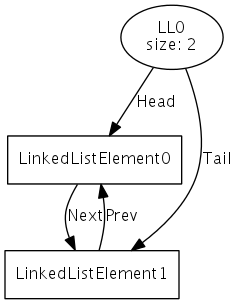
\includegraphics[width=.3\textwidth]{images/ll1}
\label{fig:inst1}
}
\hfil
\subfloat[Instance with $5$ elements for $LinkedList$]{
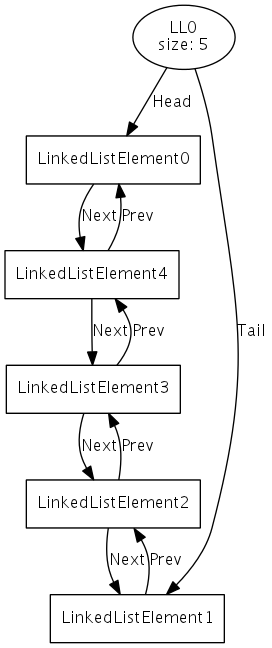
\includegraphics[width=.25\textwidth]{images/ll2}
\label{fig:inst2}}}
\caption{Examples of generated instances from Korat for $LinkedList$ class.}
\label{fig:insts}
\end{figure}

\section{Summary}
After the experimental study of the selected tools, reported in the previous subsections, it was found that PathCrawler and Pex have different
approaches regarding testcase generation. PathCrawler seems to be a very efficient tool to discover multiple
infeasible paths in C code, because it uses a mix between static and dynamic analysis. When it finds a suitable input for a function it tries to execute
collecting all the executed paths in the code.
Pex on the other side just uses static execution and it is very efficient discovering all the feasible paths in C\# methods. Pex was also used
to perform testcase generation in C\# classes, but the generated instances are too simple to perform more interesting tests. The $LinkedList$ class was written
in C\# with many management methods implemented (Add, Remove, Find,\ldots). Pex generated very simple $LinkedList$'s structures to perform automatic test generation
for each implemented method. The problem is that the generated structures does not meet the properties about Doubly Linked Lists as it can be seen in Figures \ref{fig:pexinst1} and \ref{fig:pexinst2}.
Concerning Korat, this is The tool to generate complex data structures. The freely available part of Korat show potential in expressing rules to hedge
the automatic generation of data structures.\\
In Table \ref{tab:tabcmp} we can see a brief comparison between all the experimented and mentioned tools, a more detailed conclusion is addressed in Chapter \ref{Concl}.

\begin{table}[!ht]
\centering
\begin{tabular}{|m{2.5cm}|m{1cm}|m{2cm}|m{2cm}|m{3.5cm}|m{3.5cm}|}\hline
\textbf{Name} & \textbf{Target Language} & \textbf{Type} & \textbf{Additional Input} & \textbf{Output} & \textbf{Comments}\\\hline
\textbf{PathCrawler} & C & White-box (symbolic execution) & Test vectors & Constraints about the executed paths & Too Complex\\\hline
\textbf{Pex} & C\# & White-box (symbolic execution) & -- & Unit Tests & Poor generated data instances (objects)\\\hline
\textbf{Korat} & JAVA & Black-box & Invariants written in JAVA & Graphical form of data structures (using Alloy-GraphViz) & Powerful generating valid data instances\\\hline
\end{tabular}
\caption{Comparison of experimented and mentioned tools}
\label{tab:tabcmp}
\end{table}

\begin{figure}[!ht]
\centerline{
\subfloat[Example of Pex generated $LinkedList$ instance to test $Remove$ method]{
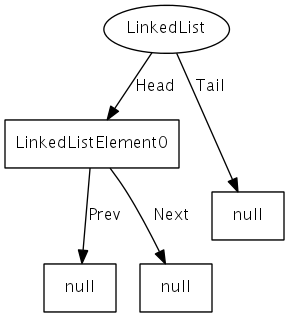
\includegraphics[width=.25\textwidth]{images/pex1}\label{fig:pexinst1}
}
\hfil
\subfloat[Example of Pex generated $LinkedList$ instance to test $Find$ method]{
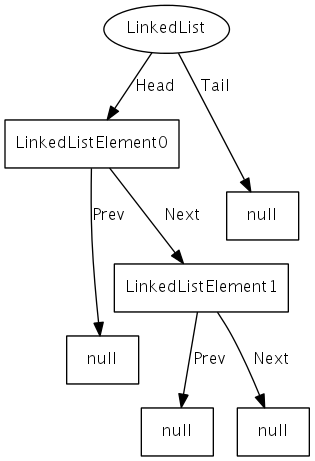
\includegraphics[width=.25\textwidth]{images/pex2}\label{fig:pexinst2}}}
\caption{Examples of generated instances from Pex for $LinkedList$ class.}\label{fig:pexG}
\end{figure}

%\section{Conclusion}\label{Concl}
%Looking for an efficient solution to automatically generate complete test sets for complex and critical C++ software,
%the state-of-the-art approaches in the area were studied and along the document some tools were introduced from methodological and experimental perspectives.
%Pex has proved to be a very powerful tool, aimed at offering a full coverage. However, the incapability for generating calling-methods sequences was a bit disappointing. 
%With Microsoft's SpecExplorer we can already
%manually call sequences of methods; maybe a combination of this feature with Pex would make Pex a perfect all-in-one testing tool regarding .NET automatic testing tools.
%Concerning Korat, the expected improvement is just to write the invariants for a class instead of the $repOK$ method, or maybe infer these invariants 
%from the existing code. Writing the $repOK$ method for very complex data structures requires some previous experience with Korat, but we think
%this is not a weakness, since the tester quickly gets used to write the $repOK$ method in Korat. The only problem is that right now we can not fully automate the process
%without human help.\\
%\indent Considering the studied tools and thinking about a full automated test generation tool, a clever composition among between Pex to ensure the maximum possible coverage, 
%Korat to generate all the valid data structures and an automatic tool to generate calls to methods combinations would be the perfect tool.\\
%
%At the end, it was proposed  an approach based on the inference of tests from a Code+OCL.
%\indent Concerning the OCL inference from C++ code, work will now be done on a tool that implements it.
%For that purpose, Frama-C will be explored, as it is well known that this tool is able to infer pre- and post-conditions\cite{moy}
%and interesting safety conditions from C source code.

\secendnote

\chapter{OCL}
\minitoc

\note{fazer um estudo sobre OCL}


\cleardoublepage
\chapter{Our Proposal and Architecture}
\minitoc
\note{onde se descrevesse a proposta e se detalhesse tecnicamente a solução arquitetónica que a poderá implementar}

\section{Generate Tests from Code+\glsentryname{OCL}}\label{proposal}
Since the Operational Simulator code is not familiar to us, regarding its implementation, it was decided to start solving this problem by inferring the \ac{UML}+\ac{OCL} from the existing code
to be able to work on a more abstract level rather than the implementation.
The idea is to extract tests from the inferred \ac{OCL}, using the Partition Analysis described
in \cite{Benattou02generatingtest} and at the same time generate tests directly from the code, using symbolic execution to complement
the specification-based generation from \ac{OCL}. The main goal is to extract as many tests as possible from a model and from the implementation 
to provide information to a feedback loop\cite{Xie03mutuallyenhancing}
test generation framework with two test prespectives, functional and structural, and from there be able to get a more refined set of tests.\\
A combination of both, symbolic execution from Pex and complex data generation from Korat, it will be designed and implemented to
generate more interesting inputs for the methods under testing.
\secendnote

\chapter{System Implemention}
\minitoc
\note{detalhes tecnicos de todas as partes novas e relevantes da arquitetura}
\secendnote

\chapter{Case Study}
\minitoc
\note{mostrar e discutir a solução proposta pela VST pra o SIMSAT}
\secendnote

\chapter{Conclusion}
\minitoc
\label{chapter-conclusion}

\section{Future work}



%bibliography
\cleardoublepage
\addcontentsline{toc}{chapter}{\bibname}
\bibliographystyle{alpha}
\bibliography{thesisBib}

\end{document}

